\documentclass[a4paper,UTF8]{article}
\usepackage{ctex}
\usepackage[margin=1.25in]{geometry}
\usepackage{color}
\usepackage{graphicx}
\usepackage{amssymb}
\usepackage{amsmath}
\usepackage{amsthm}
%\usepackage[thmmarks, amsmath, thref]{ntheorem}
\theoremstyle{definition}
\newtheorem*{solution}{Solution}
\newtheorem*{prove}{Proof}
\usepackage{multirow}
\usepackage{url}
\usepackage[colorlinks,urlcolor=blue]{hyperref}
\usepackage{enumerate}
\usepackage{float}
\setcounter{secnumdepth}{4}
\renewcommand\refname{参考文献}
%--

%--
\begin{document}
\title{\textbf{《 计算机图形学》5月说明书}}
\author{学号,姓名,\href{mailto:xxx@xxx.com}{171240511@smail.nju.edu.cn}}
\maketitle

\section{开发环境}
\begin{itemize}
\item 系统: windows 10 1809
\item Anaconda3(5.3.1): 
	\begin{itemize}
		\item python 3.7.0
		\item numpy 1.15.1
		\item pillow 5.2.0
		\item pyqt 5.9.2
	\end{itemize}
\item IDE: Spyder 3.3.1
\item 解释器: ipython 6.5.0
\end{itemize}
\section{编译运行}
CLI编译运行的命令和讲义一样: python cg\_cli.py input\_path output\_path\\
\indent GUI的运行命令: python cg\_gui.py
\section{系统功能说明}
\subsection{命令行功能}
接受两个参数, 第一个参数为指令文件的绝对路径或相对路径, 第二个参数为画布保存位置的绝对路径.
实现讲义要求所有指令, 内容格式和讲义一致.
\subsection{图形功能}
\subsubsection{界面总览}
图形界面整体情况如下图,最上面是菜单栏,可以进行设置画笔颜色等操作.\\
\indent 下面一行是编辑工具栏,可以对图元进行平移等操作.\\
\indent 左边是绘图工具栏,可以选择要绘制的图元类型及算法.\\
\indent 右边白框显示图元类型及编号, 点击可以用于选择图元.\\
\indent 下方状态栏显示当前在进行什么操作.\\
\indent 最中间的则是画布区域,可以用鼠标操作绘图.
\begin{figure}[H]
	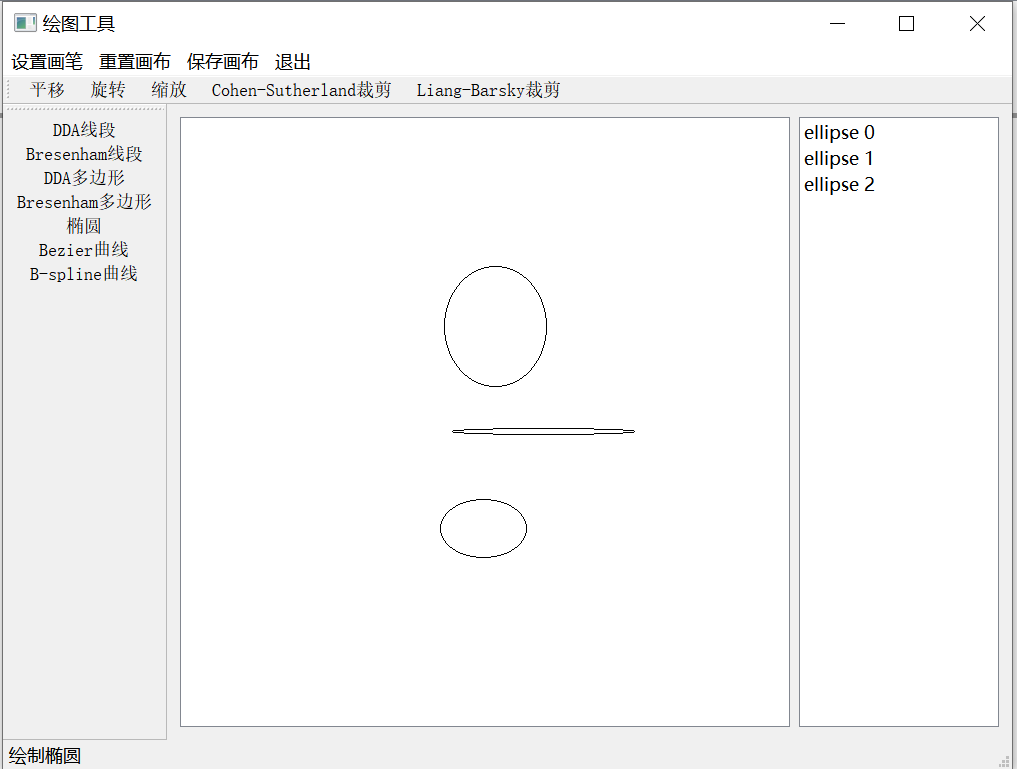
\includegraphics[width=5in,height=3in]{total.png}
\end{figure}
\subsubsection{菜单栏操作}
设置画笔颜色时点击``设置画笔"按钮,会弹出调色板,选择后即可更改画笔颜色.\\
\begin{figure}[H]
	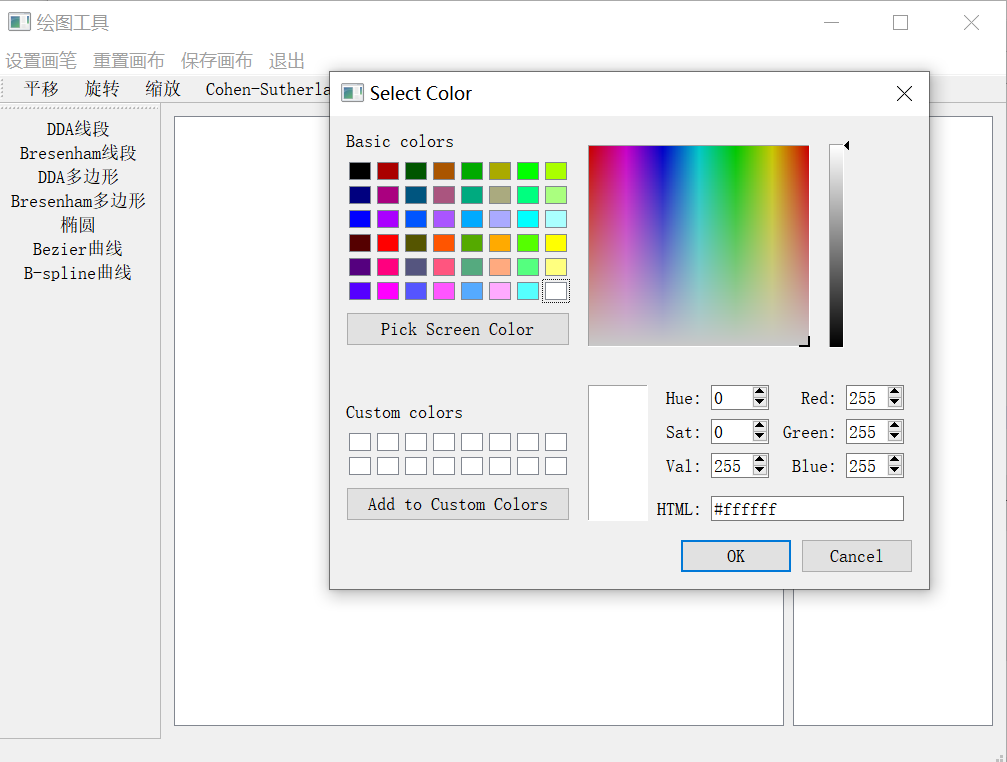
\includegraphics[width=5in,height=3in]{color.png}
\end{figure}
要设置画布大小有两种方法,一种是点击``重置画布"按钮,会连续弹出两个窗口要求输入新的x轴和y轴大小,要求x,y的范围在[100,1000]之间,不然重置无效.重置时清空画布和图元选择区\\
\indent 另一种方法是按住画布的右边框,下边框或右下边框并拖动, 这种方法不会清空画布, 但x,y的范围仍然限制 在[100,1000].
\begin{figure}[H]
	
\includegraphics[width=5in,height=3in]{reset.png}
\end{figure}
要保存画布时点击``保存画布"按钮,会弹出选择文件保存窗口,选择路径并保存即可.默认文件的格式为bmp且无法更改,文件不论命名为``name.bmp"还是``name",最终结果都是``name.bmp", 但若是命名成``name.jpg"结果就是``name.jpg".
\begin{figure}[H]
	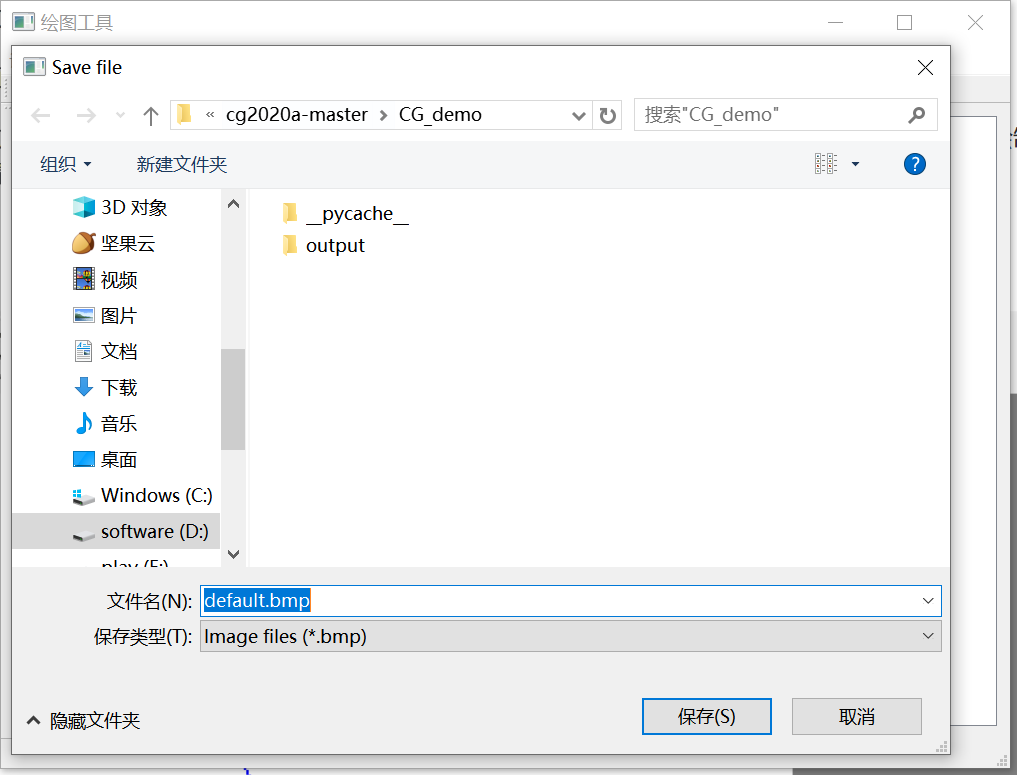
\includegraphics[width=5in,height=3in]{save.png}
\end{figure}
退出GUI界面则可以点击``退出"按钮,也可以右上角的$X$.
\subsubsection{绘图工具栏操作}
绘制线段可以点击``DDA线段"或者``Brehansem线段"按钮,会使用相应的算法,然后在画布区用鼠标点击拖动即可绘制.
\begin{figure}[H]
	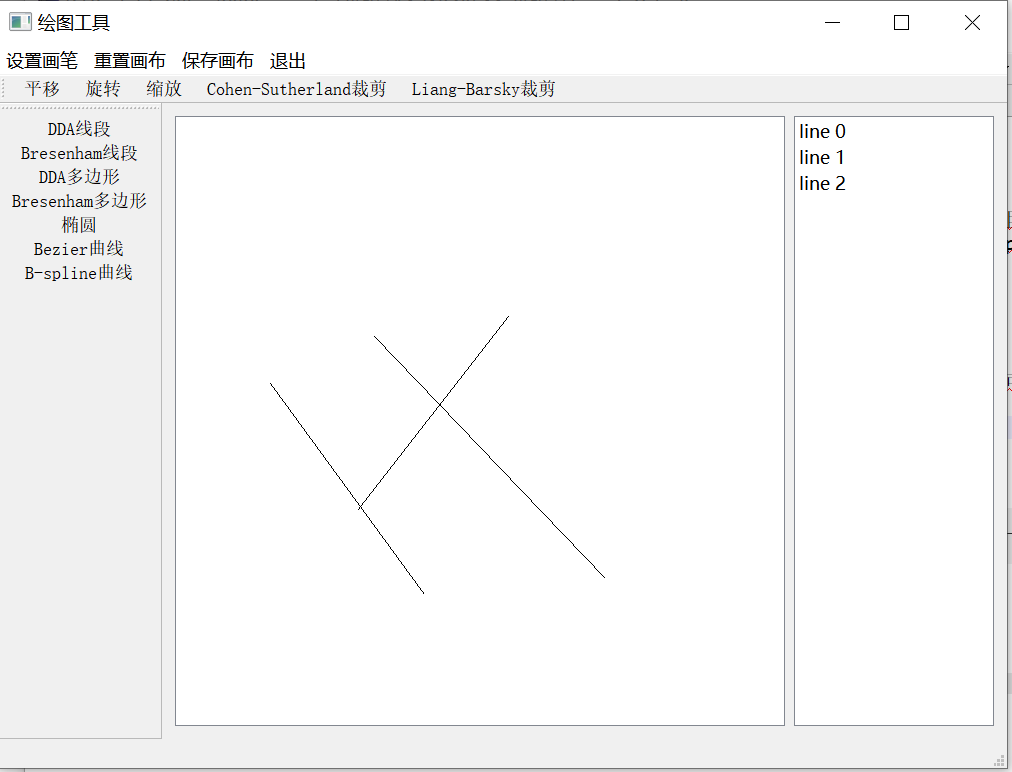
\includegraphics[width=5in,height=3in]{line.png}
\end{figure}
绘制多边形的按钮是``DDA多边形"和``Brehansem多边形",绘制时会从上一个端点向当前鼠标按住的位置画线段,直到最后一个端点的位置离起始点足够近时,松开鼠标多边形自动闭合.\\
\indent 如果多边形没有画完就去做别的事情,比如绘图或者选择图元,它仍然会自动闭合.
\begin{figure}[H]
	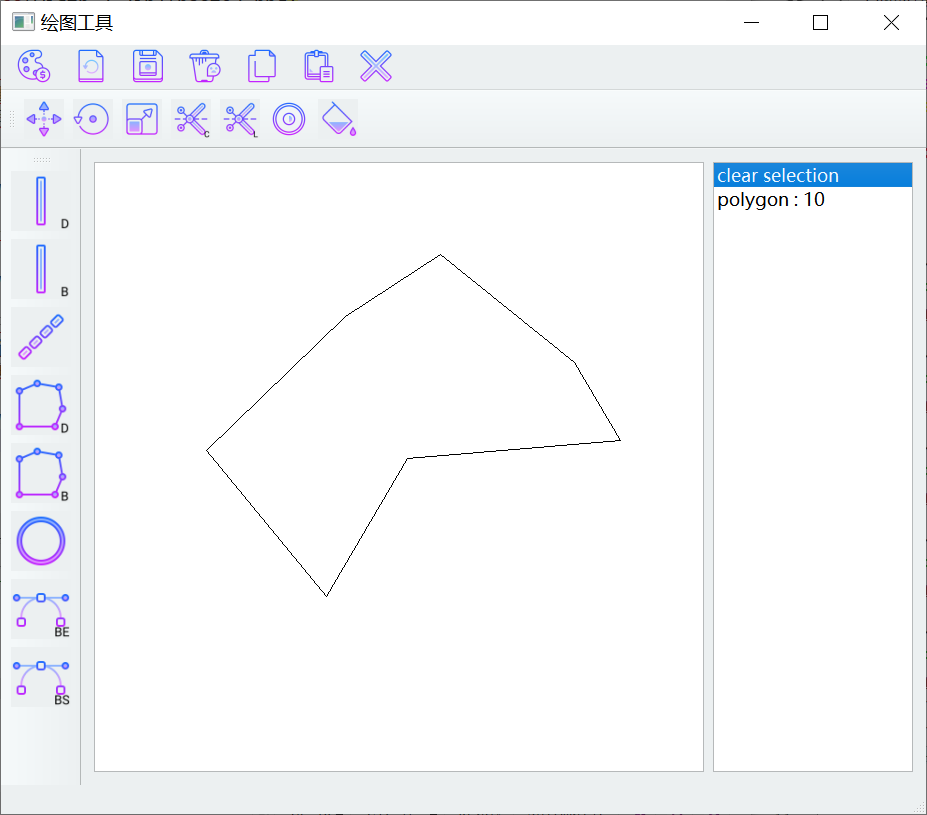
\includegraphics[width=5in,height=3in]{polygon.png}
\end{figure}
绘制椭圆的按钮是``椭圆",绘制时鼠标拖出一个不显示的矩形窗口,鼠标松开时,生成的椭圆刚好与该窗口相切.
\begin{figure}[H]
	
\includegraphics[width=5in,height=3in]{ellipse.png}
\end{figure}
绘制曲线的按钮是``Bezier曲线"和``B-spline曲线",两种算法绘制的时候,都是先鼠标拖动确定起始控制点和终止控制点,然后鼠标点击并松开的位置作为除终止点外的最新控制点.
\begin{figure}[H]
	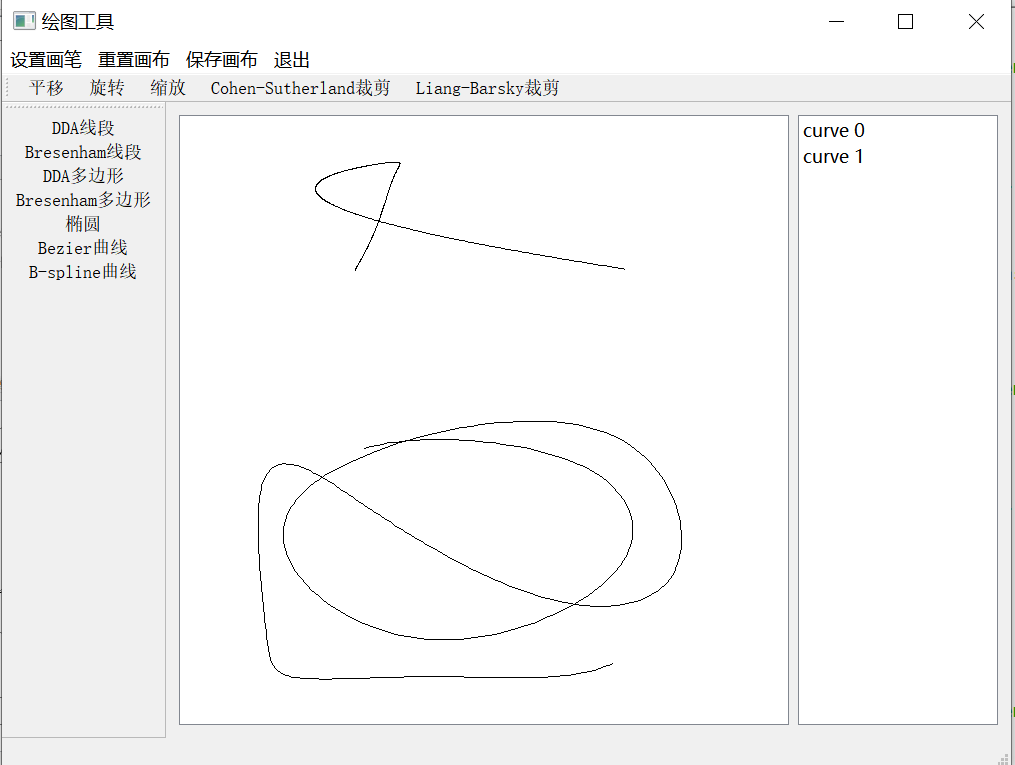
\includegraphics[width=5in,height=3in]{curve.png}
\end{figure}
\subsubsection{编辑工具栏操作}
编辑图元前需要先选中图元,只要点击右边的图元id即可选中图元,选中图元所在区域由红色方框显示.
\begin{figure}[H]
	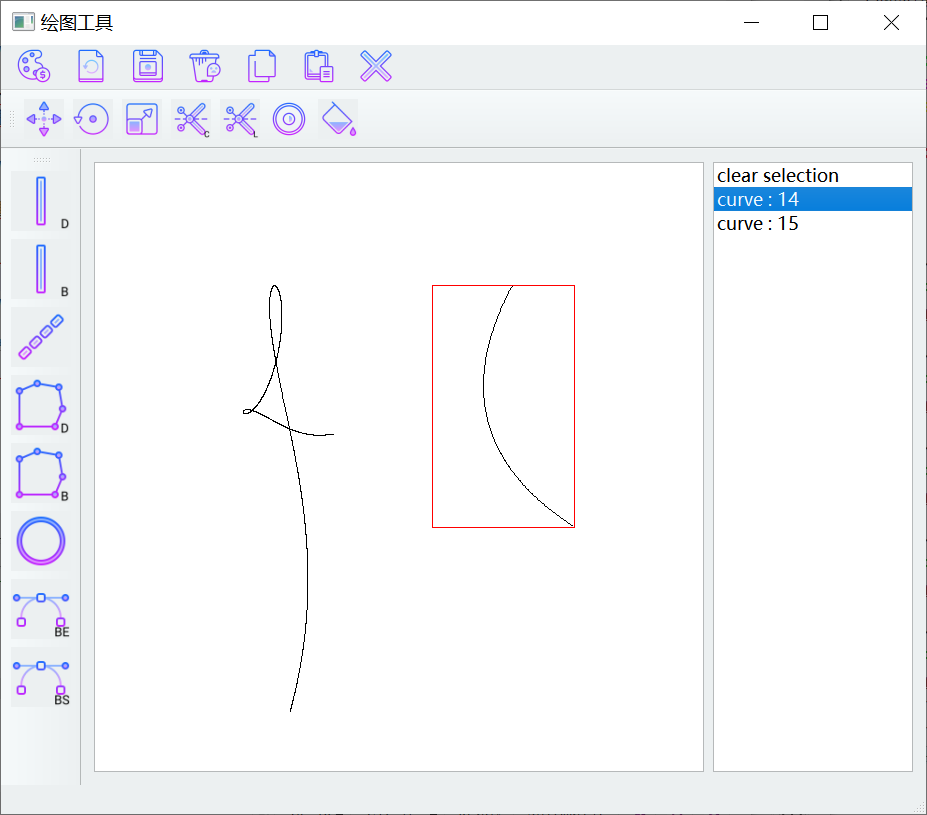
\includegraphics[width=5in,height=3in]{choose.png}
\end{figure}
平移操作只要选中图元后,点击``平移"按钮,再点击画布拖动,鼠标点击的位置是平移向量的起始点[x1,y1],鼠标拖动松开的位置是平移向量的终止点[x2,y2],平移向量[dx,dy]=[x2-x1,y2-y1].
\begin{figure}[H]
	\centering
	\begin{minipage}[t]{0.5\linewidth}
		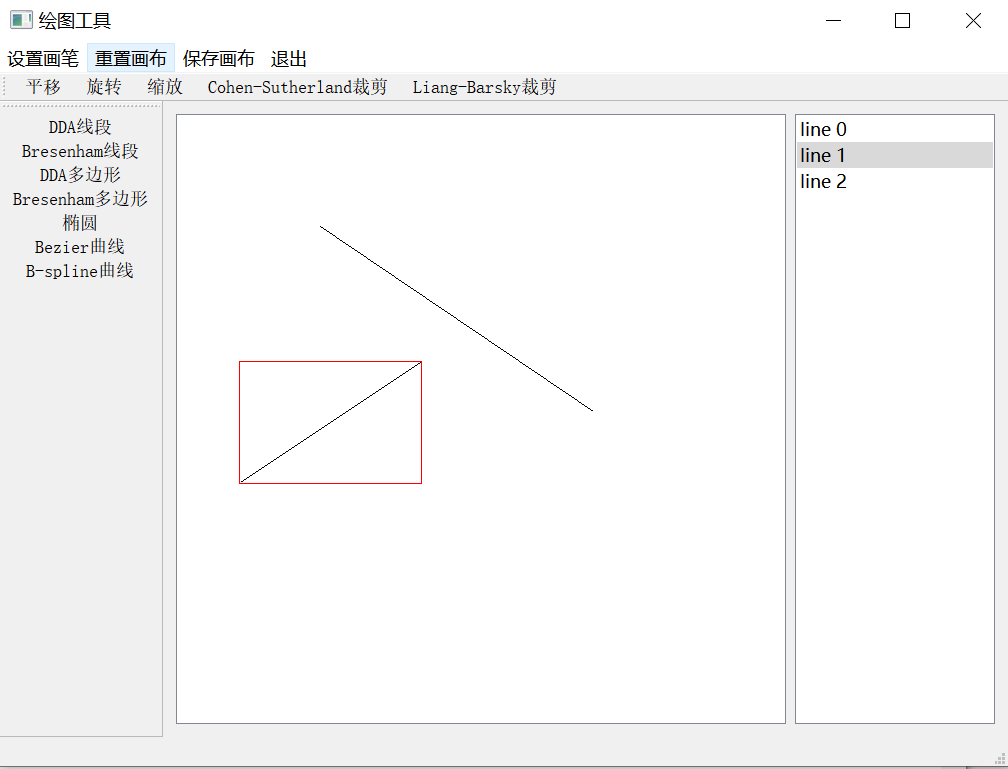
\includegraphics[width=2.2in]{translate1.png}
	\end{minipage}%
	\begin{minipage}[t]{0.5\linewidth}
		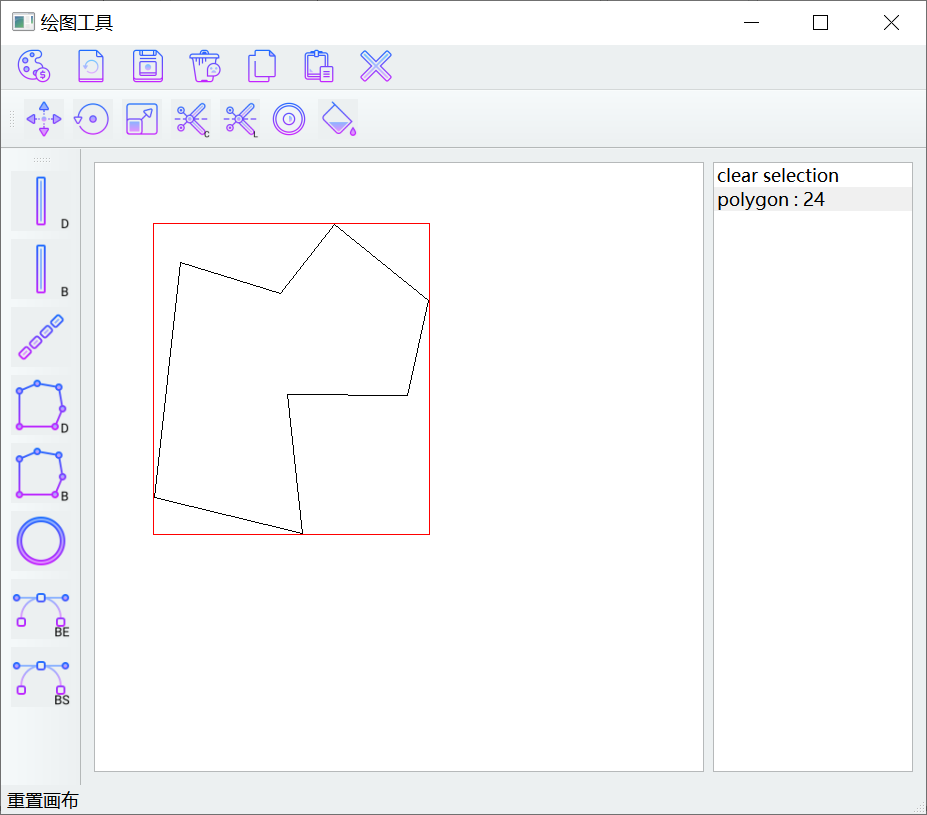
\includegraphics[width=2.2in]{translate2.png}
	\end{minipage}
\end{figure}
旋转操作先选中图元,点击``旋转"按钮,再点击画布操作.鼠标点击的第一下决定旋转中心[xr,yr],鼠标点击的第二下,按住位置和拖动松开位置的两个点与旋转中心的夹角为旋转角度.
\begin{figure}[H]
	\centering
	\begin{minipage}[t]{0.5\linewidth}
		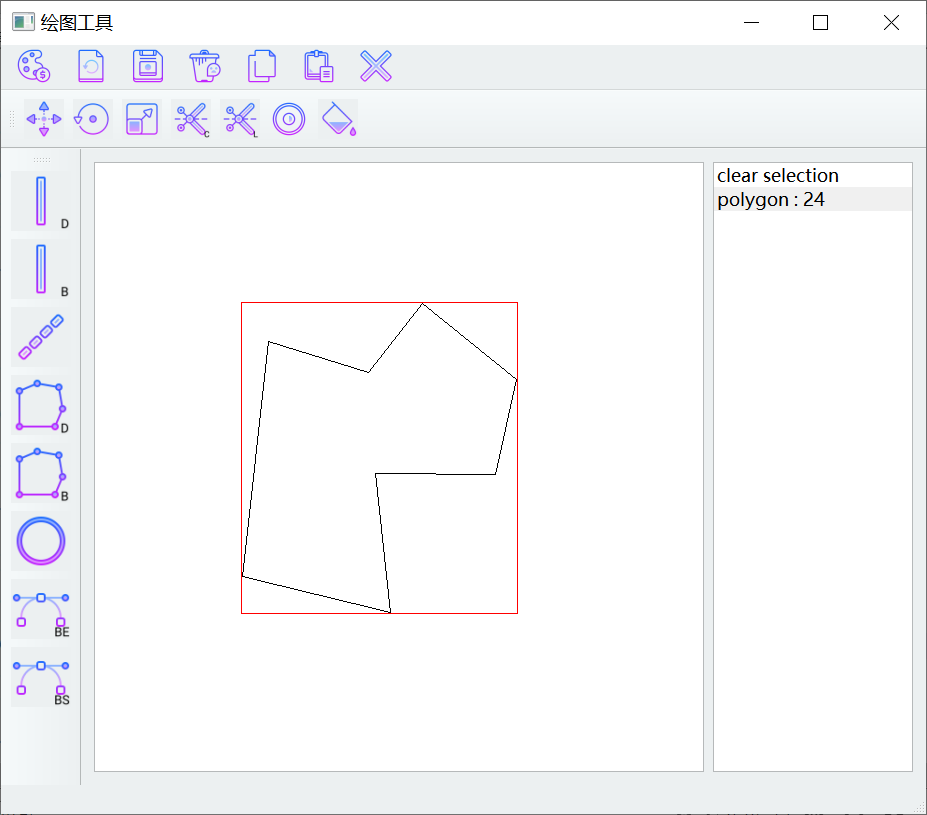
\includegraphics[width=2.2in]{rotate1.png}
	\end{minipage}%
	\begin{minipage}[t]{0.5\linewidth}
		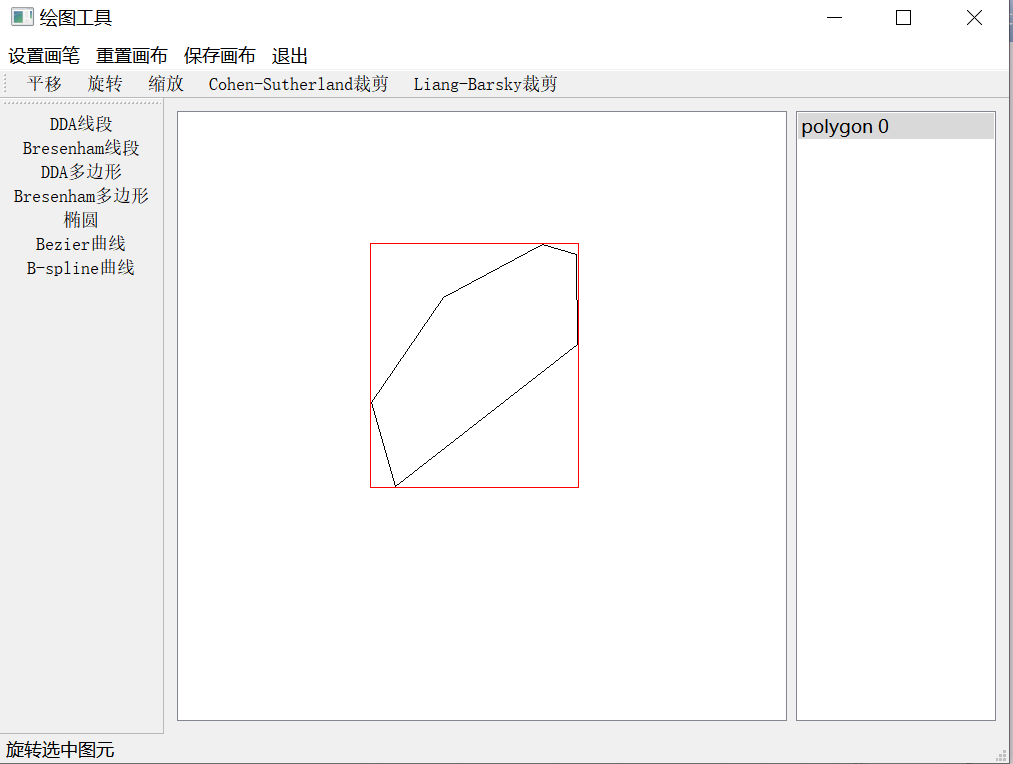
\includegraphics[width=2.2in]{rotate2.png}
	\end{minipage}
\end{figure}
缩放操作先选中图元,点击``缩放"按钮,再点击画布操作.鼠标点击的第一下决定缩放中心[xs,ys],鼠标点击的第二下,按住位置和拖动松开位置的两个点与缩放中心形成两条线段, 两条线段的x坐标比值决定缩放倍数.
\begin{figure}[H]
	\centering
	\begin{minipage}[t]{0.5\linewidth}
		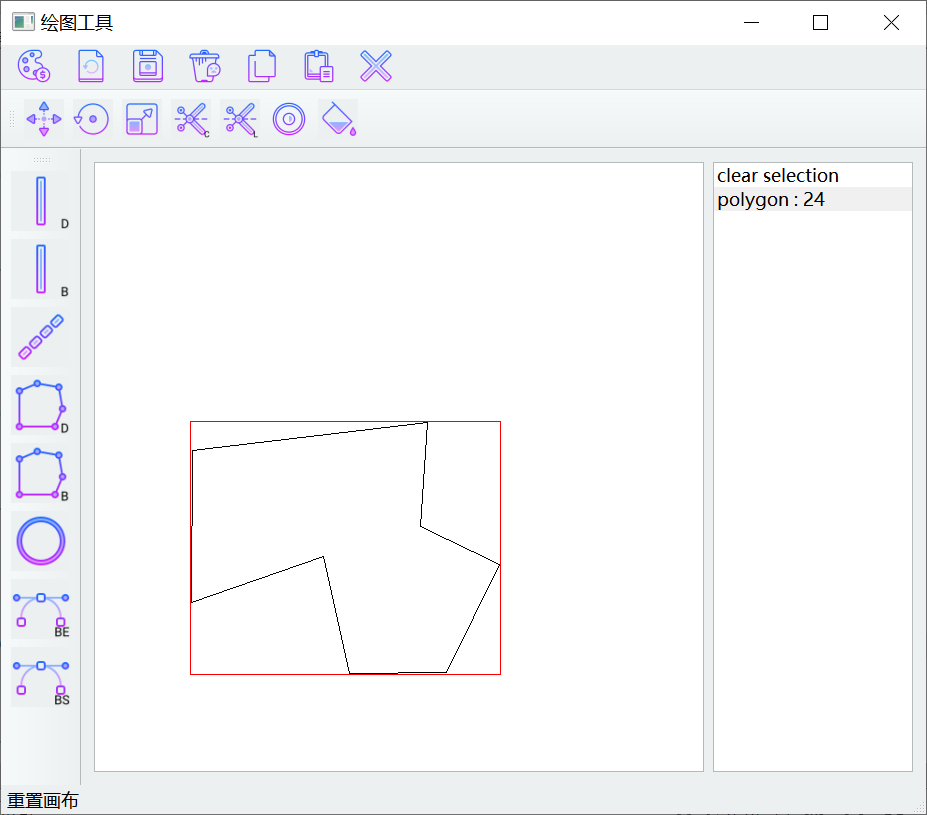
\includegraphics[width=2.2in]{scale1.png}
	\end{minipage}%
	\begin{minipage}[t]{0.5\linewidth}
		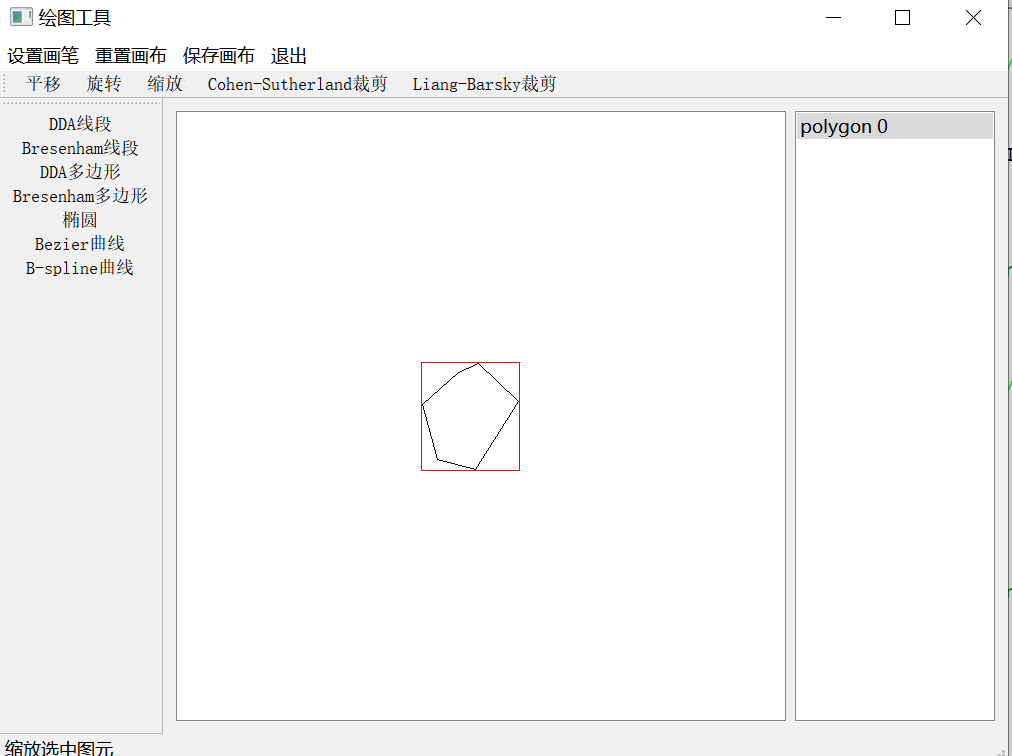
\includegraphics[width=2.2in]{scale2.png}
	\end{minipage}
\end{figure}
裁剪操作先选中线段类型图元,点击``Cohen-Sutherland裁剪"或``Liang-Barsky裁剪"按钮,再点击画布拖出裁剪窗口,松开鼠标时线段在窗口内的部分留下.\\
\indent 裁剪时窗口内线段红色高亮.\\
\indent 如果选中的图元不是线段类型,则不进行操作.\\
\indent 如果线段被裁剪没了,右边白框仍有该图元,但无法对它进行任何操作.
\begin{figure}[H]
	
\includegraphics[width=5in,height=3in]{clip.png}
\end{figure}
\end{document}